\documentclass{article}

% if you need to pass options to natbib, use, e.g.:
% \PassOptionsToPackage{numbers, compress}{natbib}
% before loading nips_2018

% ready for submission
\usepackage{nips_2018}

% to compile a preprint version, e.g., for submission to arXiv, add
% add the [preprint] option:
% \usepackage[preprint]{nips_2018}

% to compile a camera-ready version, add the [final] option, e.g.:
% \usepackage[final]{nips_2018}

% to avoid loading the natbib package, add option nonatbib:
% \usepackage[nonatbib]{nips_2018}

\usepackage[utf8]{inputenc} % allow utf-8 input
\usepackage[T1]{fontenc}    % use 8-bit T1 fonts
\usepackage{hyperref}       % hyperlinks
\usepackage{url}            % simple URL typesetting
\usepackage{booktabs}       % professional-quality tables
\usepackage{amsfonts}       % blackboard math symbols
\usepackage{nicefrac}       % compact symbols for 1/2, etc.
\usepackage{microtype}      % microtypography
\usepackage{svg}
\usepackage{amsmath}
\usepackage[ruled]{algorithm2e}

\title{Parallel Joint PPO}

% The \author macro works with any number of authors. There are two
% commands used to separate the names and addresses of multiple
% authors: \And and \AND.

% Using \And between authors leaves it to LaTeX to determine where to
% break the lines. Using \AND forces a line break at that point. So,
% if LaTeX puts 3 of 4 authors names on the first line, and the last
% on the second line, try using \AND instead of \And before the third
% author name.

\author{
  Albert Ge\thanks{Equal contribution.} \\
  Department of Computer Science\\
  Cranberry-Lemon University\\
  San Jose, CA 95129 \\
  \texttt{lbertge@gmail.com} \\
  %% examples of more authors
  %% \And
  %% Coauthor \\
  %% Affiliation \\
  %% Address \\
  %% \texttt{email} \\
  %% \AND
  %% Coauthor \\
  %% Affiliation \\
  %% Address \\
  %% \texttt{email} \\
  %% \And
  %% Coauthor \\
  %% Affiliation \\
  %% Address \\
  %% \texttt{email} \\
  %% \And
  %% Coauthor \\
  %% Affiliation \\
  %% Address \\
  %% \texttt{email} \\
}

\begin{document}
% \nipsfinalcopy is no longer used

\maketitle

\begin{abstract}
  I implement a method for parallelizing a jointly-trained PPO algorithm on the
  Gym Retro Sonic games, on a single GPU and processor. Tantamount to this algorithm were improved memory efficiency and getting enough sleep, both of which were realized and successfully resolved. Parallel Joint PPO achieves about a 3x speedup on a machine with a GTX 1080 and 32GB of RAM. A working implementation can be found at the repository \url{https://github.com/lbertge/retro-noob/tree/master/joint-ppo}.
\end{abstract}

\section{Introduction}

The OpenAI Retro Contest \cite{DBLP:journals/corr/abs-1804-03720} is an online competition aimed at applying transfer-learning algorithms on custom-built Sonic levels, using released Sonic games (\textsc{SonicTheHedgehog-Genesis}, \textsc{SonicTheHedgehog2-Genesis}, \textsc{SonicAndKnuckles3-Genesis}). On submission, an algorithm is packaged into a Docker container and executed remotely for evaluation on a set of test levels. 

\subsection{Background}

In 2018, OpenAI released its Gym Retro repository which enables reinforcement-learning research on a slew of \textsc{Sega-Genesis} games via their standard Gym environment. 

\subsection{Previous Work}

Previous work on transfer-learning for the \textsc{SonicTheHedgehog} franchise has suggested that a jointly-trained Proximal Policy Optimization \cite{DBLP:journals/corr/SchulmanWDRK17} (PPO) algorithm generalizes well to the test set. 
Joint PPO is identical to normal PPO, with the difference being trained \emph{simultaneously} on all environments. This means that, after playing through each level once, the algorithm produces a list of gradients obtained from each level, averages them using the arithmetic mean, and applies the resulting gradient to the policy. To accomplish this, The authors use a cluster of GPUs to execute the training in parallel, with each GPU assigned to a single level from one \textsc{SonicTheHedgehog} game. This requires resources which is generally above the average machine learning enthusiast's budget, which may also exceed that of this paper's author; thus, this paper seeks to find another, more efficient method for joint training, which is capable of running on more modest hardware.

Reinforcement learning is perhaps no stranger to hardware constraints; previous work on parallelizing the TRPO algorithm \cite{DBLP:journals/corr/SchulmanLMJA15} has demonstrated that distributed RL training can result in speedup by as much as 5x over training \cite{frans2016parallel}, which was also done over a home PC. While the work in this paper takes a remarkably similar approach to parallelizing TRPO, an important difference is that joint PPO trains over a set of gym environments, which faces its own memory-constraint issues to be able to accomodate for the results from all gym environments. Thus, this paper details and resolves a number of technical challenges involving parallelizing joint PPO.

\section{PPO}
PPO as an algorithm attempts to produce the same results as TRPO while using only first-order optimization methods, which is significantly less complex than TRPO. At its core, PPO minimizes the following objective:
\[
  L^{CLIP} = \hat{\mathbb{E}_t}[\textnormal{min}(r_t(\theta)\hat{A}_t, \textnormal{clip}(r_t(\theta),1-\epsilon, 1+\epsilon)\hat{A}_t)]
\]
where $r_t(\theta)$ is the probability ratio between the current stochastic policy $\pi_{\theta}$ and its previous policy $\pi_{\theta_{\textmd{old}}}$ for action $a_t$ and state $s_t$, or 
\[r_t(\theta) = \frac{\pi_{\theta}(a_t | s_t)}{\pi_{\theta_{\textnormal{old}}}(a_t | s_t )}\] and $\hat{A}_t$ is the advantage function. Recall that the advantage function approximates how optimal it is to take an action over all other actions in a given state. To get an intuitive sense for this equation, consider two scenarios: one in which the advantage is positive (i.e., good action) and one in which it is negative (bad action).
\begin{itemize}
  \item If the advantage is positive, the only notable situation is when ratio $r_t(\theta)$ is greater than 1 (the action under the current policy is more probable than the previous policy). This would introduce a multiplying factor (>1) to $\hat{A}_t$. To prevent this factor from becoming too large, the ratio is clipped by a constant hyperparameter $\epsilon$ such that the advantage never exceeds a multiple of $1 + \epsilon$, and prevents greedy optimization of making the action too probable.
  \item If the advantage is negative, and the ratio $r_t(\theta)$ is less than 1 (action is less probable), the objective is clipped such that the advantage never exceeds a multiple of $1-\epsilon$. Since the objective is negative, This places an upper bound on the objective function, and it forces the policy to not overupdate and make the action too improbable. 
\end{itemize}
In both cases the clipping objective prevents the policy being updated in such a way that capitalizes excessively on improvement. Otherwise, if the policy ratio worsens the behavior, the clipping has no effect, and the objective function penalizes the policy as normal.

\section{Architecture}

A diagram of the system architecture used can be found in Figure 1, and a description of the algorithm can be found at Algorithm \ref{alg:joint}. Each iteration begins in the process with id 0, which will be referred to as the master process. The master process spawns worker processes (pids 1, 2, 3). Every process, including the workers, creates its own Tensorflow context, and models are synchronized via message passing through a blocking queue, for concurrency safety. 

During training, each worker evaluates its model one of 47 \textsc{SonicTheHedgehog} Gym environments specified in the training set, producing a tuple of experiences obtained during $T$ timesteps. Experiences here is defined as observations (raw input), advantage estimates, values, and negative log probabilities. These experiences are passed back to the master process, and gradients are produced for each set of experiences for $K$ epochs and $M$ minibatches. Finally, the gradients are averaged and the resulting gradients is applied to the master's copy of the model, and re-synchronized with the other worker processes.

\begin{figure}[htbp]
  \centering
  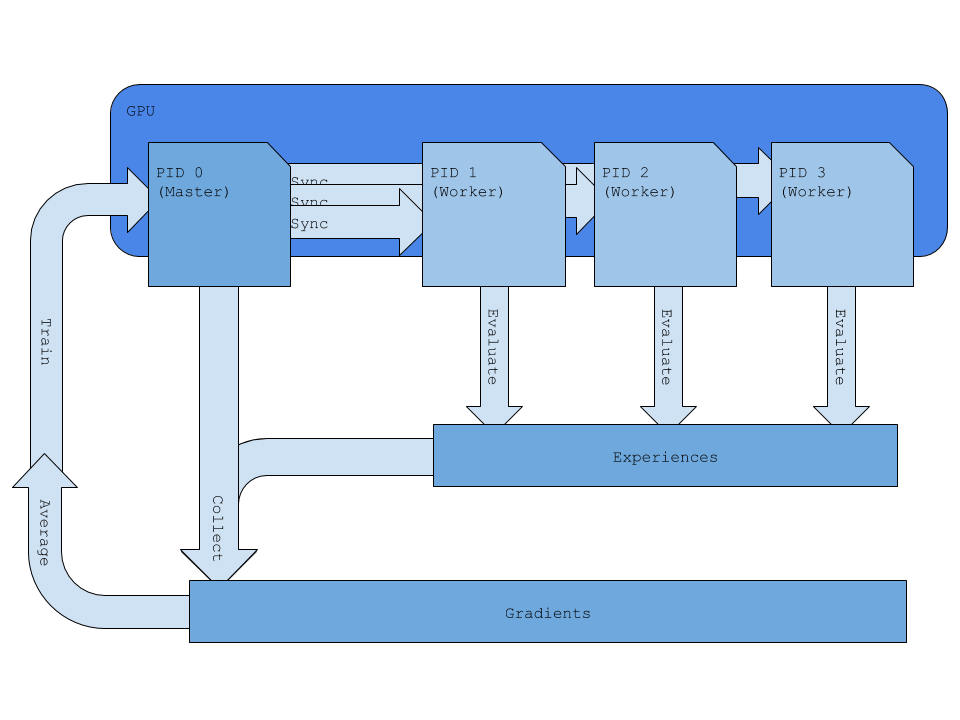
\includegraphics[width=\columnwidth]{arch.png}
  \label{fig:arch}
  \caption{System Architecture for parallelizing joint PPO. Each node in the diagram represents a physical state, and each directed edge refers to an action performed in, or on that physical state. For example, inside of process with \texttt{pid 0} (Master), experiences are collected and gradients are computed/averaged. }
\end{figure}

\begin{algorithm}
  \For{iteration=1,2}{
    Enqueue 47 environments in queue \\
    \While{\textnormal{queue} not empty}{
      Run policy $\pi_{\theta_{\textnormal{old}}}$ for T timesteps \\
      experiences.append(advantage estimates, neglogpacs, observations)

    }
    \For{experience in \textnormal{experiences}}{
      compute gradients for $K$ epochs with minibatch size $M$ (optimizing for $L_t^{CLIP+VF+S}$)
    }
    Average gradients \\
    Apply gradients\\
  }
  \caption{Parallel Joint PPO}
  \label{alg:joint}
\end{algorithm}

\pagebreak

\subsection{Preventing memory leaks}

The model architecture was specifically designed to prevent memory leaking, and an overview of this design is presented in Figure 2. Two source of memory leaks were discovered, both of which were successfully resolved:
\begin{itemize}
  \item During the \textbf{Sync} step of Figure 2, the master's model with those of the workers, the weights are pickled and sent over the blocking queue to each worker. Each worker will then load the weights by calling \texttt{tf.assign}, which is a Tensorflow operation (op) that overwrites the values in the existing graph with those obtained from the queue. However, Tensorflow ops are permanent while the context session is active, meaning that with each iteration, \texttt{tf.assign} ops will be continually added, leading to about 30MB additional memory per worker process.
    \subitem To resolve this, a single \texttt{placeholder} Tensor object and \texttt{assign} op is created on graph initialization. Since the placeholder object is only initialized once, and can accomodate array objects of variable size and shape, the weights are first placed inside the placeholder, which in turn executes the assign op to map the weights into the model. Thus, this method prevents runaway memory usage, capping a Worker's memory requirements to about 3GB.
  \item The second issue arises in the \textbf{Collect} step of Figure 2, when attempting to average gradients from all levels together. An important note is that the \texttt{apply\_gradients} op appears to \textit{consume} the gradient Tensor objects during execution. Thus, if no \texttt{apply\_gradients} op immediately follows the \texttt{compute\_gradients} op, the Tensor objects become orphaned in the graph, and it is difficult to explicitly free without killing the entire context session. In this particular case, running the model on each level environment's experiences results in a separate list of gradients, leading to about an additional 600MB per gradient Tensor.
    \subitem The solution is similar to the first scenario. In this instance, a set of \texttt{tf.Variable} objects are initialized, which are reused when computing each environment's gradients. \texttt{tf.Variable} is used instead of \texttt{tf.placeholder} because the gradients are aggregated and averaged outside of the Tensorflow context session, which would allow each Worker process to separately compute each gradient, rather than just evaluating and collecting experiences. Due to the poor author's time and budget constraints, that work remains slightly out of the scope of this paper, and hopefully remains on the horizon for future work.
\end{itemize}

Table ~\ref{sample-table} shows a list of hyperparameters used for training the algorithm.

\begin{figure}[htbp]
  \centering
  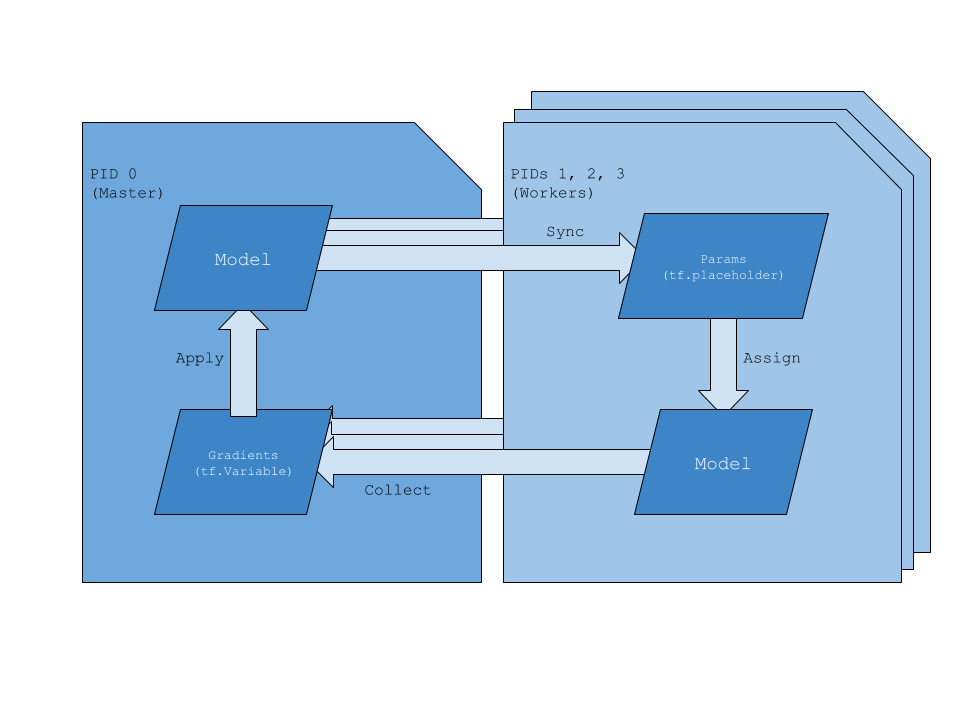
\includegraphics[width=\columnwidth]{graph.png}
  \label{fig:graph}
  \caption{Model Architecture for Joint PPO. Here, each parallelogram refers to a node (or group of nodes) inside of the Tensorflow's execution graph. Each light blue arrow represents a Tensorflow operation performed. Both memory leaks occur when transferring data between Tensorflow sessions, i.e. when syncing the master's model with the those of the worker's, and when collecting experiences/averaging gradients from the workers back to the master process.}
\end{figure}

\section{Performance}

Resolving the two memory issues reduces the requirements from unbounded to about 14GB for the master process, and 3GB for each Worker process. Additionally, with 3 worker processes, the parallelized PPO algorithm can process over 21 million total timesteps in about 9 hours, which is about a 3x speedup over a single process (about 7 million timesteps in 9 hours). 

\section{Sleep}

Sleep is really important, and vital for being able to think through technical challenges without going around in circles.

\begin{table}
  \caption{Hyperparameters for Joint PPO training}
  \label{sample-table}
  \centering
  \begin{tabular}{ll}
    \toprule
    \cmidrule(r){1-2}
    Hyperparameter    & Value \\
    \midrule
    Workers & 3 \\
    Horizon & 4500 \\
    Epochs & 4 \\
    Minibatch size & 1125 \\
    Discount $\gamma$ & 0.99 \\
    GAE $\Lambda$ & 0.95 \\
    Clipping $\epsilon$ & 0.2 \\
    Entropy coeff $\epsilon$ & 0.2 \\
    Reward scale & 0.01 \\
    \bottomrule
  \end{tabular}
\end{table}

\section{Conclusion}

This paper documents and explains the issues encountered during implementing a parallelized version of jointly-trained PPO, and the solutions found to overcome them. In particular, memory leak issues were the core issue due to the processing of many Gym environments in parallel, which were resolved by reusing heavily-trafficked nodes and ops inside of the Tensorflow execution graph. Furthermore, which is evaluated on the \textsc{SonicTheHedgehog} games on the Sega-Genesis. The parallelized algorithm can have a speedup of about 3x over its single-processor counterpart.

\subsection{Future Work}
There still remains much future work to be done, such as actually evaluating the agent and confirming that it has improved performance over its meta-learning-less counterpart, normal PPO. Initial results look promising and will be released in an updated version of this paper.

\subsubsection*{Acknowledgments}

Thanks to the OpenAI team for releasing and maintainining the Gym Retro environments, the baselines PPO algorithm implementation, and for giving the the author two months of wild speculation about how to improve agent evaluation. 

\medskip 

\small

\bibliography{biblio}
\bibliographystyle{apalike}

\end{document}